\documentclass[tikz,border=2mm]{standalone}
\usetikzlibrary{3d,}         % 'canvas is...' options
\usetikzlibrary{perspective} % isometric view

\begin{document}
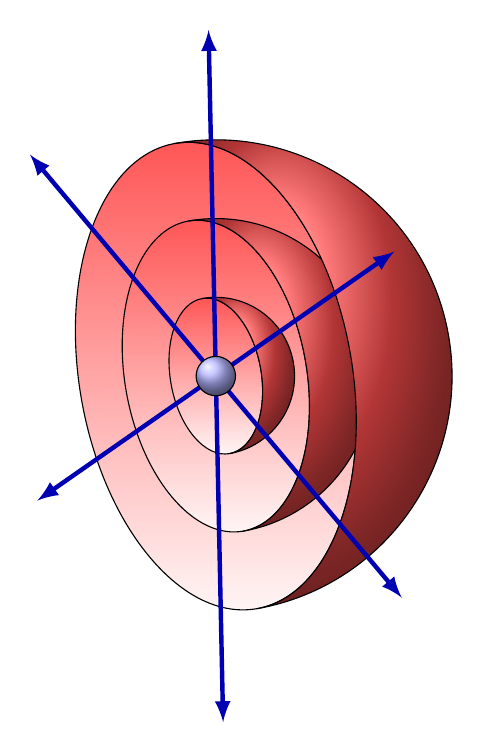
\begin{tikzpicture}[isometric view,rotate=-20]
% sphere, inner
\foreach\i in {3,2,1}
  \draw[canvas is yz plane at x=0,top color=red!70] (0,0) circle (\i);
% sphere, outer
\foreach\i in {1,2,3}
  \draw[shading=ball,ball color=red!70] (120:\i cm) arc (120:-60:\i cm)
                       {[canvas is yz plane at x=0] arc (225: 45:\i)};
% rays
\foreach\i in {0,60,120}
  \draw[canvas is yz plane at x=0,blue!70!black,ultra thick,latex-latex]
      (\i:4.5) -- (\i+180:4.5);
\draw[shading=ball,ball color=blue!30] (0,0) circle (0.25cm);
\end{tikzpicture}
\end{document}